\chapter{Non-Terrestrial Networks}
\label{ch:non_terrestrial_networks}

\glspl{ntn} represent a groundbreaking approach in wireless communication, utilizing aerial and space-based platforms to deliver connectivity services. These platforms can operate at varying altitudes, from a few hundred meters to several kilometers above ground, offering key advantages over traditional terrestrial networks, such as expanded coverage, increased capacity, and greater flexibility.

\glspl{ntn} provide a promising solution to meet the rising demand for wireless access in remote and underserved areas. By leveraging aerial and space platforms, \glspl{ntn} can extend the reach of conventional terrestrial networks, offering connectivity where traditional infrastructure is either difficult or impossible to deploy. These platforms are available in several configurations, including high-altitude platforms, low-earth orbit satellites (e.g., \glspl{leo}), and geostationary satellites (e.g., \glspl{geo}), each with distinct benefits in terms of coverage, capacity, and latency, making them suitable for various use cases. In \cref{fig:ntn_types}, we illustrate the different types of \glspl{ntn} based on altitude and platform type as well as their interaction with other network elements such as ground stations, \glspl{uav}, \gls{iot} devices, etc.

\section{Geostationary Satellites}

\glspl{geo} operate at an altitude of approximately \SI{35786}{\kilo\meter} above the Earth's equator. These satellites maintain a fixed position relative to the Earth’s surface, as they orbit at the same rate as the planet's rotation. \glspl{geo} offer extensive coverage, often spanning entire continents, and are widely used for telecommunications, broadcasting, and weather monitoring.

Compared to \glspl{leo}, \glspl{geo} offer broader coverage and higher capacity, making them ideal for applications like direct-to-home television, satellite radio, and broadband internet access. Their capacity to cover large regions makes \glspl{geo} integral to global communications infrastructure.

A key advantage of \glspl{geo} is their ability to support high-capacity services for many users, making them valuable for broadcasting live events, such as sports and concerts, or delivering high-definition video content worldwide. As a fundamental part of the global media and communication ecosystem, \glspl{geo} are expected to continue playing a vital role in providing connectivity to remote and underserved regions.

\section{Low-Earth Orbit Satellites}

\glspl{leo} are satellites operating at altitudes between \SI{160}{\kilo\meter} and \SI{2000}{\kilo\meter} above the Earth. Orbiting at high speeds, these satellites provide global coverage, making them ideal for delivering connectivity to remote and underserved regions. \glspl{leo} offer several advantages over traditional geostationary satellites, including lower latency, higher capacity, and reduced infrastructure costs.

Deployed in constellations consisting of hundreds or thousands of satellites, \glspl{leo} work together to provide continuous coverage. These satellites communicate through inter-satellite links, allowing data to be relayed seamlessly across the constellation. \glspl{leo} are well-suited for delivering broadband internet access in areas where traditional infrastructure is difficult to establish.

One of the primary advantages of \glspl{leo} is their low latency, enabling real-time communication and supporting applications that require minimal delay, such as online gaming, video conferencing, and autonomous vehicle systems. Additionally, \glspl{leo} offer high-speed internet connectivity to users in remote locations, granting access to online services, educational platforms, and e-commerce opportunities. As a critical part of the emerging \gls{ntn} ecosystem, \glspl{leo} are expected to play a key role in bridging the global digital divide.

\section{High-Altitude Platforms}

High-altitude platforms operate at altitudes ranging from a few hundred meters to several kilometers above the Earth. These platforms may consist of balloons, airships, or \glspl{uav}. They provide several benefits compared to traditional terrestrial networks, including broader coverage, increased capacity, and lower infrastructure costs. High-altitude platforms can be deployed swiftly to offer connectivity in remote or underserved areas, making them an effective tool for reducing the digital divide.

Additionally, high-altitude platforms can provide temporary connectivity in disaster-stricken regions or during large-scale events. Rapid deployment allows emergency responders to coordinate efforts efficiently. They can also extend the coverage of existing networks in rural areas, where conventional infrastructure is costly or challenging to install.

Advances in \gls{uav} technology have enabled the development of autonomous high-altitude platforms equipped with \gls{lte} or \gls{5g} base stations, flying at altitudes of up to \SI{20}{\kilo\meter}. These platforms cover vast areas and support a range of applications, making them ideal for remote and underserved locations where deploying traditional infrastructure is not practical.

\begin{figure}
  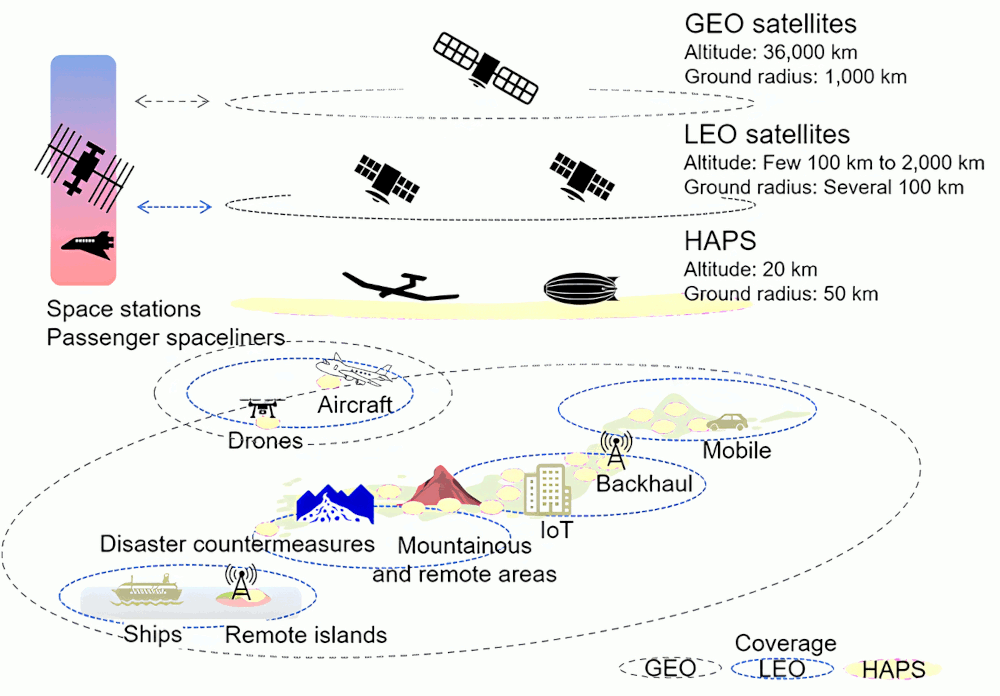
\includegraphics{non_terrestrial_networks_types.png}
  \caption{Types of \glspl{ntn} based on altitude and platform type. High-altitude platforms, low-earth orbit satellites, and geostationary satellites interact with other network elements to provide connectivity services. \autocite{alertifyAirbusNTT}}
  \label{fig:ntn_types}
\end{figure}
